\section{Auswertung}
\label{sec:Auswertung}
Die Messunsicherheiten des folgenden Kapitels wurden mit \textit{Python} unter Verwendung des Paketes \textit{scipy} \cite{scipy} bestimmt. Sie folgen aus der gaußschen
Fehlerfortpflanzung
\begin{equation}
  \label{eqn:Gauss}
  \Delta F = \sqrt{\sum_i\left(\frac{\symup{d}F}{\symup{d}y_i}\Delta y_i \right)^2}.
\end{equation} 

\subsection{Bestimmung der Winkelrichtgröße und des Eigenträgheitsmoments der Drehachse}
\label{subsec:A_Apparatenkonstanten}
Bevor mit dem eigentlichen Versuch begonnnen werden kann, müssen die Winkelrichtgröße $D$ der Feder und das Eigenträgheitsmoments $I_D$ der Drehachse ermittelt werden. 
Erstere kann mithilfe der Messwerte aus \autoref{tab:Winkelricht} durch Anwendung von \autoref{eqn:Winkelrichtgröße} bestimmt werden. Neben den Messwerten finden sich die jeweiligen 
Werte der Winkelrichtgröße in der genannten Tabelle.
\begin{table}
  \centering
  \caption{Messdaten zur Bestimmung der Winkelrichtgröße zum festen Abstand $a = \qty{20}{\centi\metre}$}
  \label{tab:Winkelricht}
  \begin{tabular}{S[table-format = 3.0] S[table-format = 1.3] S}
    \toprule
    {$\phi \mathbin{/} °$} & {$F \mathbin{/} \unit{\newton}$} & {$D \mathbin{/} \unit{\newton\metre\per\radian}$} \\
    \midrule
     20 & 0.025 & 0.029 \\
     30 & 0.045 & 0.034 \\
     40 & 0.067 & 0.038 \\
     50 & 0.1   & 0.046 \\
     60 & 0.124 & 0.047 \\
     70 & 0.145 & 0.047 \\
     80 & 0.17  & 0.049 \\
     90 & 0.25  & 0.064 \\
    100 & 0.27  & 0.062 \\
    110 & 0.3   & 0.063 \\
    \bottomrule
  \end{tabular}
\end{table}
Durch Mittelung der experimentellen Werte für die Winkelrichtgröße ergibt sich der Mittelwert $D = \qty{0.048 +- 0.012}{\newton\metre\per\radian}$.

Zur Bestimmung des Eigendrehmoments der Drehachse wird \autoref{eqn:Schwingungsdauer} betrachtet. Für das Quadrat der Schwingungsdauer $T$ ergibt sich
durch einsetzen des Gesamtträgheitsmoments $I = I_D + I_\text{Zylinder}$ unter Verwendung des Satzes von Steiner \eqref{eqn:Steiner}
\begin{equation}
  \label{eqn:I_D}
  T^2 = \frac{4\pi^2}{D}\left(I_D + 2I_\text{Z,h} + 2 m a^2) \right)
\end{equation}
mit der Masse $m = \qty{261.2}{\gram}$, dem Trägheitsmoment $I_\text{Z,h}$ eines zylinderförmigen Gewichtes und dem Abstand $a$ der Zylinder zur Drehachse. $I_\text{Z,h}$
berechnet sich dabei nach der Gleichung für einen horizontalen Zylinder aus \autoref{fig:Trägheitsmomente}.
Die Gleichung stellt eine Geradengleichung der Form $f(x) = mx +b$ mit $f(x) = T^2(a^2)$ dar. In \autoref{fig:plot} sind die 
Quadrate der Messwerte für die Schwingungsdauer $T$ zum Abstand $a$ zur Drehachse aufgeführt. 
\begin{figure}
  \centering
  \includegraphics[width=0.8\textwidth]{plot.pdf}
  \caption{Graph der Quadrate der Messwerte und Ausgleichsgerade der linearen Regression. \cite{matplotlib}}
  \label{fig:plot}
\end{figure}
Eine lineare Regression mittels \textit{scipy} \cite{scipy} ergibt die Geradenparameter $m = \qty{732 +- 5}{\second\squared\per\metre\squared}$ und 
$b = \qty{5.62 +- 0.27}{\second\squared}$. Ein Koeffizientenvergleich von \autoref{eqn:I_D} und der Geradengleichung ergibt 
\begin{equation*}
  b = \frac{4\pi^2}{D}(I_D + 2I_\text{Z,h}),
\end{equation*}
woraus sich das Eigenträgheitsmoment $I_D$ bestimmen lässt. Mit dem Durchmesser $d = \qty{4.5}{\centi\metre}$ und der Höhe $h = \qty{2}{\centi\metre}$ der zylinderförmigen
Gewichte folgt $I_D = \qty{6.2 +- 1.6}{\gram\square\metre}$. Dieser Wert liegt eine Größenordnung über den im Folgenden zu bestimmenden Trägheitsmomenten, was nicht der 
Wahrheit entsprechen kann, da das Trägheitsmoment der Drehachse selbst sehr viel kleiner ist. Näheres hierzu findet sich in \autoref{sec:Diskussion}. Der wahre Wert von
$I_D$ wird für weitere Rechnungen als vernachlässigbar gering angenommen.

\subsection{Bestimmung des Trägheitsmoments des Zylinders}
\label{subsec:A_zylinder}
Der verwendete Zylinder hat eine Höhe $h = \qty{10.09}{\centi\metre}$ und einen Durchmesser $d = \qty{9.83}{\centi\metre}$. Die Masse des Zylinder beträgt $m = \qty{367.7}{\gram}$.
Die Schwingungsdauer wurde zehn Mal gemessen mit jeweils fünffacher Periodendauer. Die Messwerte können \autoref{tab:einfacheKörper} entnommen werden. 
Zur Berechnung des Trägheitsmoments werden die Einzelmessungen zunächst auf eine Schwingungsperiode gemittelt. Anschließend wird der Mittelwert aller Messwerte gebildet.
\begin{table}
    \centering
    \caption{Messwerte der Schwingungsdauern von Zylinder und Kugel.} 
    \label{tab:einfacheKörper}
    \begin{tabular}{c c}
        \toprule
        ${5}T_{z} \mathbin{/} \unit{\second}$ & ${5}T_k \mathbin{/} \unit{\second}$ \\
        \midrule
        3.81 & 9.29 \\
        3.76 & 9.20 \\
        3.77 & 9.43 \\
        3.78 & 9.37 \\
        3.74 & 9.24 \\
        3.85 & 9.40 \\
        3.82 & 9.32 \\
        3.84 & 9.21 \\
        3.86 & 9.28 \\
        3.77 & 9.30 \\
        \bottomrule 
    \end{tabular}
\end{table}
Die mittlere Periodendauer des Zylinders beträgt $\overline{T}_z = \qty{0.760+-0.008}{\second}$.
Mittels \autoref{eqn:I_K} kann das experimentelle Trägheitsmoment des Zylinders $I_{z,\text{exp}}$ berechnet werden. Durch einsetzen der Werte ergibt sich $I_{z,\text{exp}} = \qty{0.70+-0.18}{\gram\metre\squared}$.
Der Theoriewert $I_{z,\text{theo}}$ des Trägheitsmoments eines Zylinders lässt sich nach der Formel für $I_z$ berechnen, welche \autoref{fig:Trägheitsmomente} entnommen werden kann.
Durch Einsetzen der Abmessungen des Zylinders ergibt sich $I_{z,\text{theo}} = \qty{0.444}{\gram\metre\squared}$.

\subsection{Bestimmung des Trägheitsmoments der Kugel}
\label{subsec:A_kugel}
Die verwendete Kugel hat einen Durchmesser von $d_k = \qty{14.72}{\centi\metre}$ und eine Masse von $m_k = \qty{1170.3}{\gram}$. Die Messwerte zur Periodendauer der Kugel
können \autoref{tab:einfacheKörper} entnommen werden. Wie schon in \autoref{subsec:A_zylinder} wird auch hier der Mittelwert zur Berechnung des Trägheitsmoments
verwendet. Die mittlere Periodendauer der Kugel ist $\overline{T}_k = \qty{1.861+-0.016}{\second}$. Das experimentelle Trägheitsmoment $I_{k,\text{exp}}$ der Kugel 
lässt sich gemäß \autoref{eqn:I_K} berechnen. Dadurch ergibt sich $I_{k,\text{exp}} = \qty{4.2+-1.1}{\gram\metre\squared}$. Der Theoriewert des Trägheitsmoments einer Kugel
kann durch die Gleichung $I_{k,\text{theo}} = \frac{2}{5}mr^2$ berechnet werden, welche \autoref{fig:Trägheitsmomente} zu entnehmen ist.
Mit den gemessenen Größen ergibt sich $I_{k,\text{theo}} = \qty{2.53}{\gram\metre\squared}$. 

\subsection{Bestimmung des Trägheitsmoments der Holzpuppe}
\label{subsec:A_holzpuppe}
Das Trägheitsmoment der Holzpuppe wird im Folgendem für zwei unterschiedliche Stellungen der Puppe bestimmt. Zuvor werden die Maße der einzelnen Gliedmaßen der Modellpuppe ausgewertet.
Alle Gliedmaßen werden als Zylinder genähert.
\begin{table}
  \centering
  \caption{Messdaten zur Bestimmung der Körpermodellierung. $d_k$ beschreibt den Durchmesser des Kopfes. Weiter beschreibt der Index a den Arm, r den Rumpf und b das Bein der Puppe.} 
  \label{tab:holzpuppe}
  \begin{tabular}{S S S S}
      \toprule
      $\unit{d_k\per\centi\metre}$ & $\unit{d_a\per\centi\metre}$ & $\unit{d_r\per\centi\metre}$ &  $\unit{d_b\per\centi\metre}$ \\
      \midrule
      2.61 & 1.30 & 3.86 & 1.92 \\
      2.86 & 1.38 & 3.76 & 1.91 \\
      2.90 & 1.40 & 3.55 & 1.80 \\
      2.83 & 1.46 & 3.00 & 1.60 \\
      2.66 & 1.20 & 3.52 & 1.56 \\
      2.21 & 1.37 & 3.73 & 1.60 \\
           & 1.47 & 4.00 & 1.70 \\
           & 1.23 & 4.22 & 1.62 \\
           & 1.12 &      & 1.40 \\
           & 1.27 &      & 1.30 \\
      \bottomrule 
  \end{tabular}
\end{table}
\autoref{tab:holzpuppe} zeigt die Messwerte der Durchmesser der einzelnen Körperteile. Aus diesen wird jeweils ein Mittelwert gebildet.
Die Maße und Massen der einzelnen Gliedmaßen sind \autoref{tab:Maße_Puppe} zu entnehmen.
\begin{table}
  \centering
  \caption{Maße und errechnetes Gewicht der als Zylinder genäherten Gliedmaßen der Holzpuppe.} 
  \label{tab:Maße_Puppe}
  \begin{tabular}{l S[table-format = 2.2] S[table-format = 1.2]@{${}\pm{}$} S[table-format = 1.2] S[table-format = 2.1] @{${}\pm{}$} S[table-format = 2.1]}
      \toprule  
       & {Höhe $h \mathbin{/} \unit{\centi\metre}$} &\multicolumn{2}{c}{Radius $r \mathbin{/} \unit{\centi\metre}$} & 
       \multicolumn{2}{c}{Masse $m \mathbin{/} \unit{\gram}$} \\
      \midrule
      {Kopf}  &  4.14 & 1.34 & 0.13 & 18   & 4   \\
      {Arm}   & 12.91 & 0.66 & 0.06 & 13.6 & 2.5 \\
      {Rumpf} &  9.84 & 1.85 & 0.18 & 82   & 1   \\
      {Bein}  & 12.42 & 0.82 & 0.10 & 20   & 4   \\
      \bottomrule 
  \end{tabular}
\end{table}
Die einzelnen Massen können bestimmt werden, indem der prozentuale Anteil des genäherten Volumens der Gliedmaßen mit der Gesamtmasse $m = \qty{167.2}{\gram}$ multipliziert wird.
Das Volumen der Zylinder berechnet sich dabei nach $V = \pi r^2h$.

\begin{figure}
  \centering
  \caption{Verschiedene Stellungen der Holzpuppe, welche auf der Drillachse montiert ist.}
  \label{fig:D_subfig}
  \begin{subfigure}{0.4\textwidth}
      \centering
      \caption{Stellung 1}
      \label{fig:D_Holzpuppe1}
      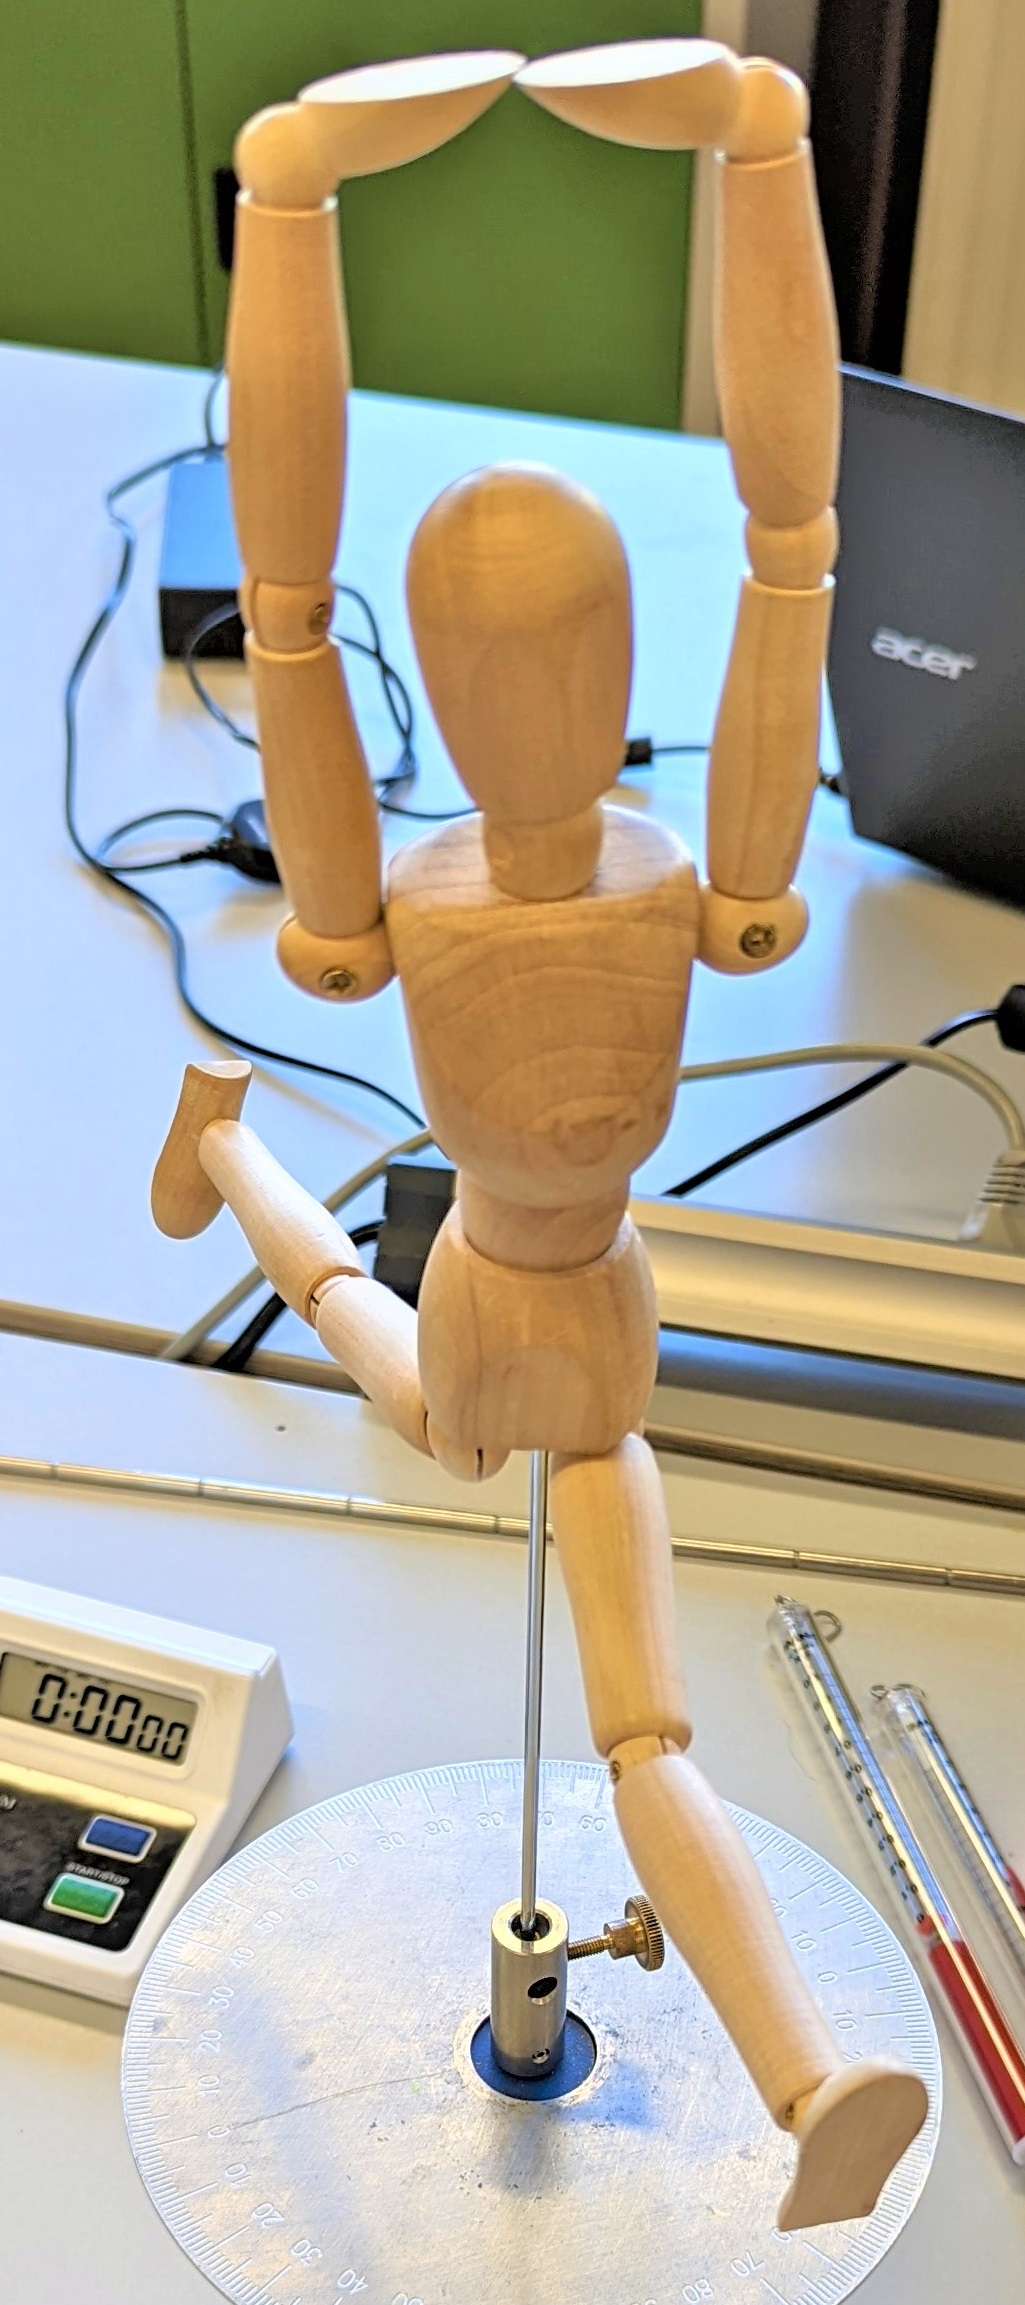
\includegraphics[width=0.65\textwidth]{content/Ballet3.jpg}
  \end{subfigure}
  \hfill
  \begin{subfigure}{0.48\textwidth}
      \centering
      \caption{Stellung 2}
      \label{fig:D_Holzpuppe2}
      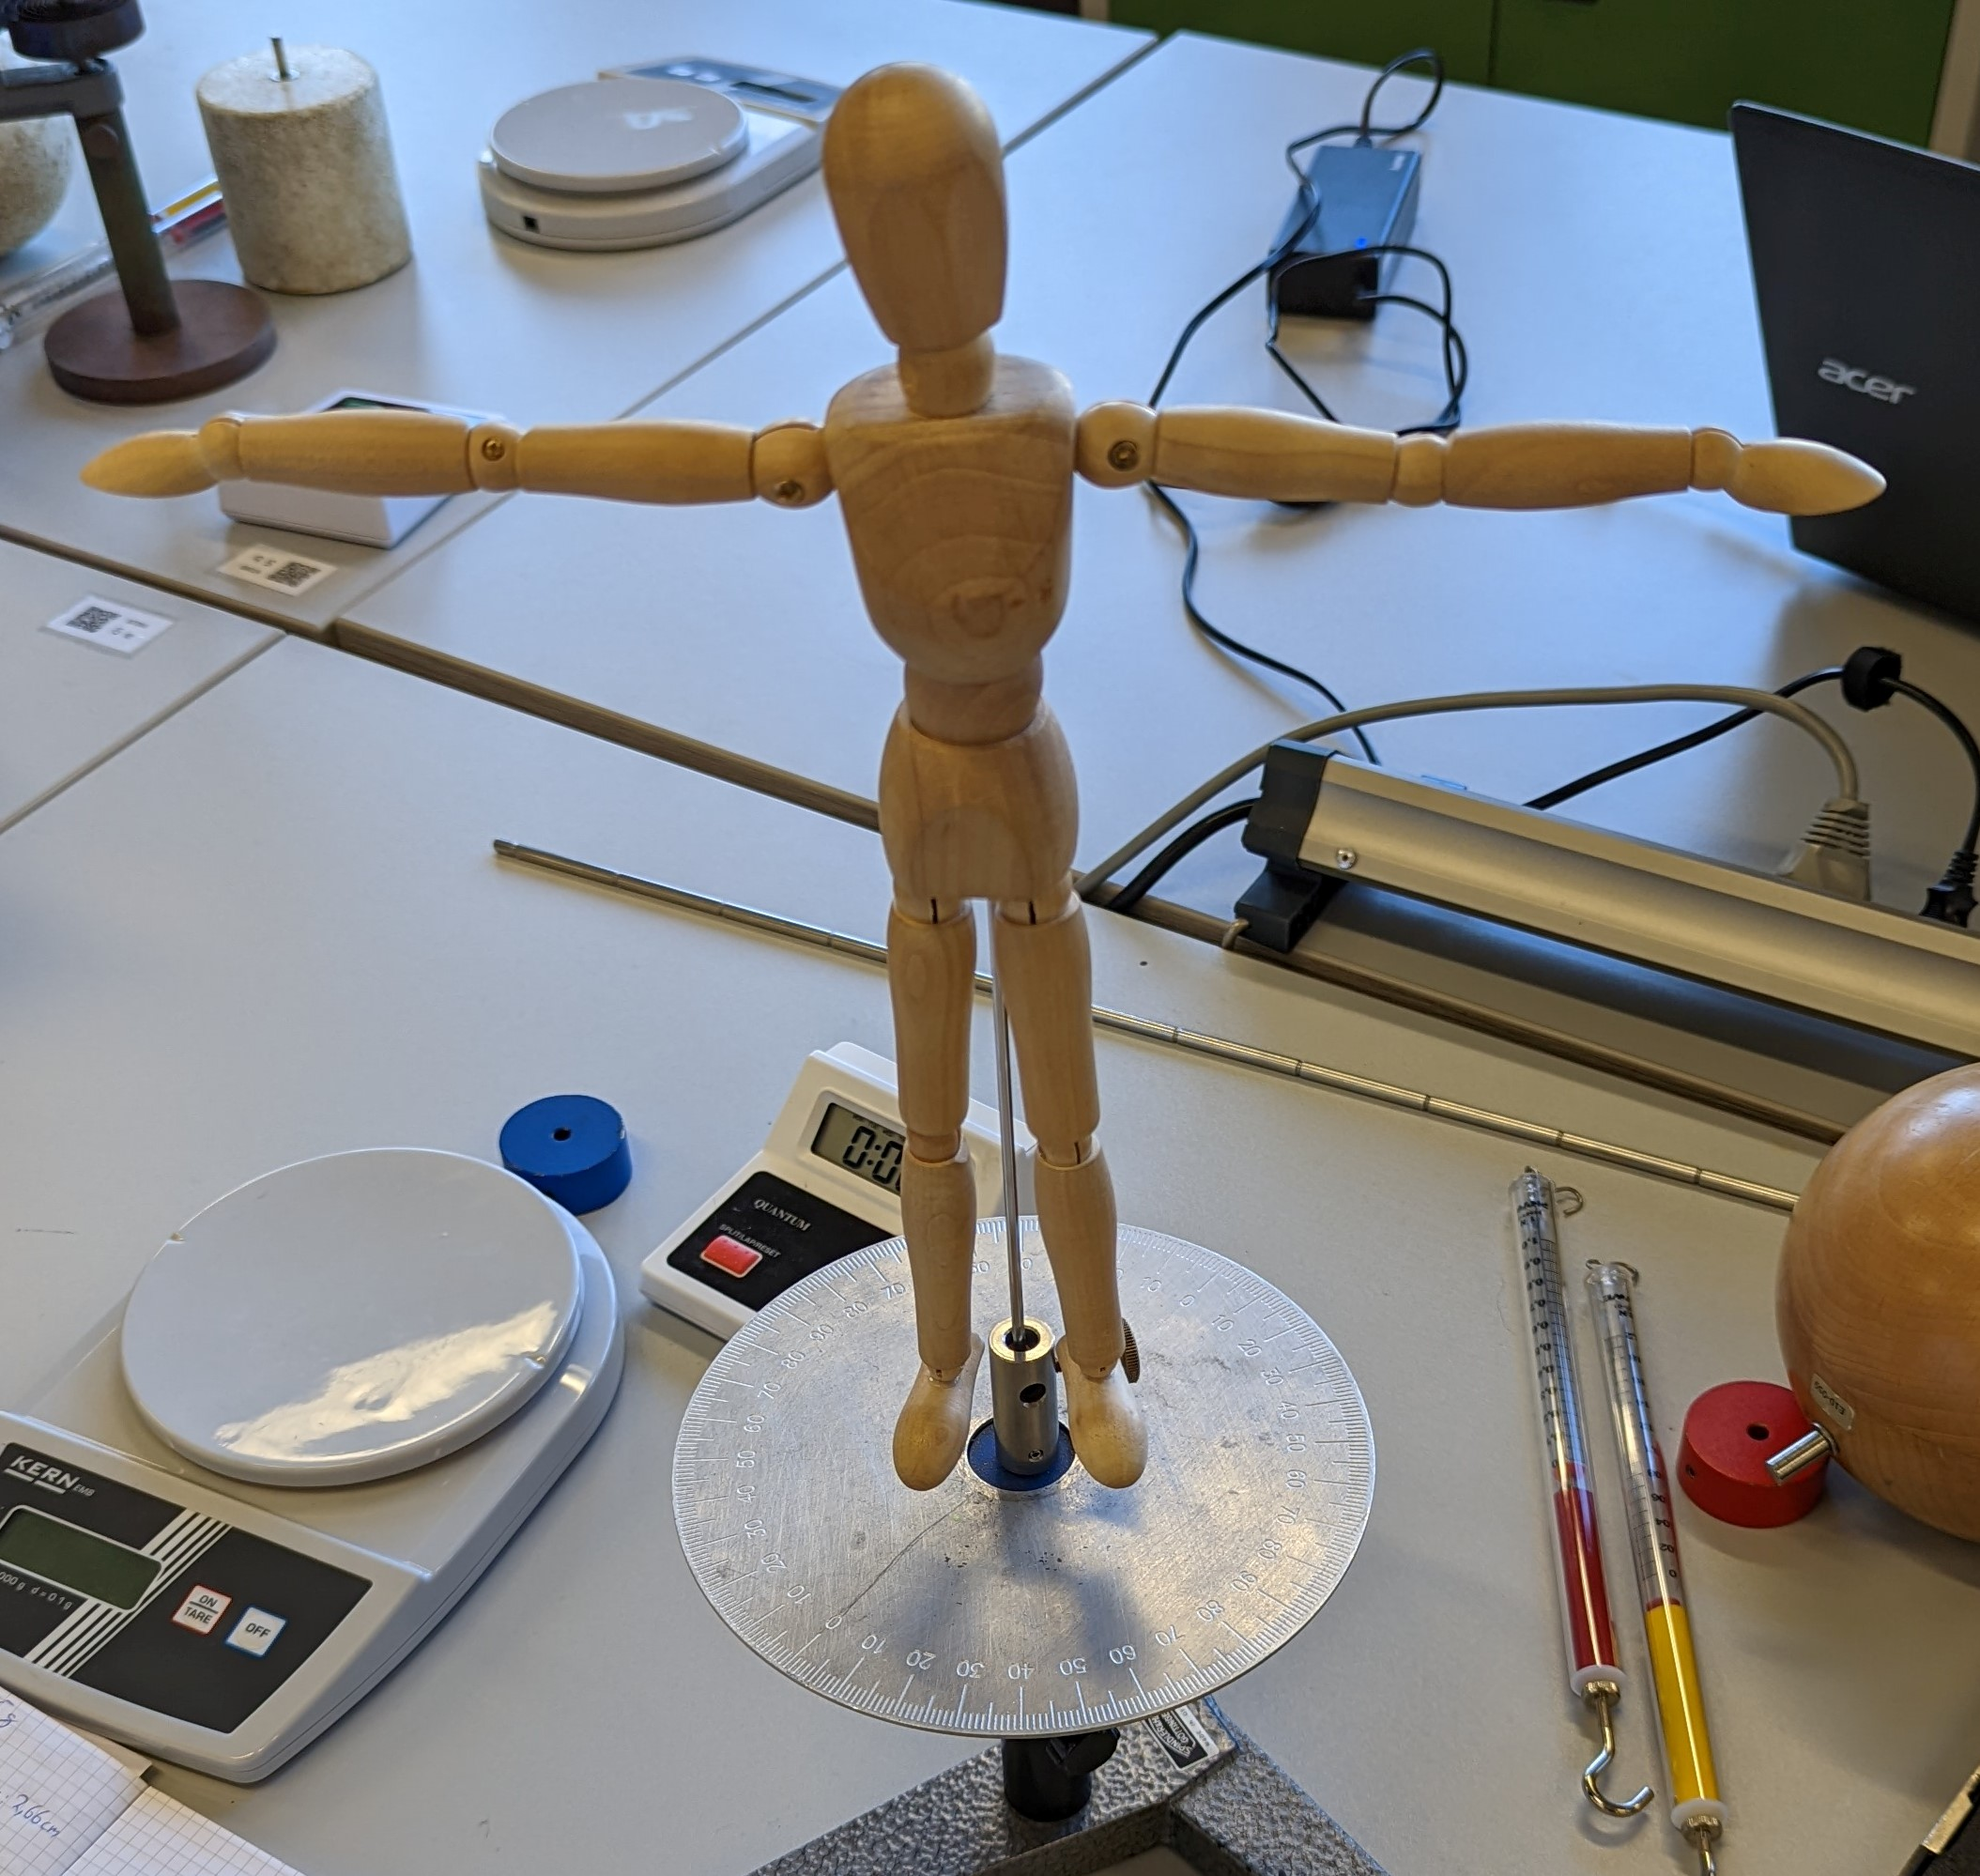
\includegraphics[width=0.8\textwidth]{content/T_Pose3.jpg}
  \end{subfigure}    
\end{figure}

\subsubsection{Trägheitsmoment der ersten Stellung}
\label{subsubsec:A_ballet}
Die erste Stellung der Figur ist in \autoref{fig:D_Holzpuppe1} zu sehen. Zunächst werden die gemessenen Schwingungsdauern, welche \autoref{tab:T_Holzpuppe} 
entnommen werden können, gemittelt. 
\begin{table}
  \centering
  \caption{Messwerte der Schwingungsdauern der Holzpuppe.}
  \label{tab:T_Holzpuppe}
  \begin{tabular}{S[table-format = 1.2] S}
    \toprule
    ${5}T_{1} \mathbin{/} \unit{\second}$ & ${5}T_{2} \mathbin{/} \unit{\second}$ \\
    \midrule
    3.81 & 3.13 \\
    3.86 & 3.17 \\
    3.91 & 3.12 \\
    3.92 & 3.14 \\
    3.74 & 3.15 \\
    3.77 & 3.31 \\
    3.70 & 3.21 \\
    3.80 & 3.20 \\
    3.52 & 3.20 \\
    3.53 & 3.24 \\
    \bottomrule
  \end{tabular}
\end{table}
Der Mittelwert einer Schwingungsperiode ergibt sich zu $\overline{T}_1 = \qty{0.751+-0.028}{\second}$.
Mit diesem Wert ergibt sich nach \autoref{eqn:I_K} $I_{1\text{,exp}} = \qty{0.684+-0.180}{\gram\metre\squared}$ für das experimentell bestimmte Trägheitsmoment der Puppe in Stellung 1. 
Der Theoriewert des Trägheitsmomentes ergibt sich durch die Gleichungen aus \autoref{fig:Trägheitsmomente} und den Satz von Steiner \eqref{eqn:Steiner}. 
Dazu werden zunächst die Trägheitsmomente der einzelnen Körperteile berechnet, welche anschließend addiert werden.
Die Einzelträgheitsmomente können \autoref{tab:einzelträgheitsmomente} entnommen werden.
\begin{table}
  \centering
  \caption{Einzelträgheitsmomente der Holzpuppe.} 
  \label{tab:einzelträgheitsmomente}
  \begin{tabular}{l c @{${}\pm{}$} l c @{${}\pm{}$} l}
      \toprule
      & \multicolumn{2}{c}{Stellung 1} & \multicolumn{2}{c}{Stellung 2} \\
      \cmidrule(lr){2-3}\cmidrule(lr){4-5}
       & \multicolumn{2}{c}{$\unit{I_{1,\text{theo}}\per\micro\gram\metre\squared}$} & \multicolumn{2}{c}{$\unit{I_{2,\text{theo}}\per\micro\gram\metre\squared}$} \\
      \midrule
      {Kopf} & 1.6 & 0.6 & 1.6 & 0.6 \\
      {Arme} & 8.9 & 1.9 & 113 & 19 \\
      {Rumpf} & 14 & 4 & 14 & 4 \\
      {Beine} & 106 & 22 & 2.8 & 0.6 \\
      \bottomrule 
  \end{tabular}
\end{table}
Das theoretische Gesamtträgheitsmoment der Modellpuppe in der Stellung 1 beträgt $I_{1\text{,theo}} = \qty{0.246+-0.040}{\gram\metre\squared}$.
\subsubsection{Trägheitsmoment der zweiten Stellung}
\label{subsubsec:A_tpose}
Wie zuvor wird ebenfalls der Mittelwert der Periodendauer in Stellung 2 gebildet. Dieser beträgt $\overline{T}_2 = \qty{0.637+-0.012}{\second}$. Mit diesem Wert kann erneut mittels \autoref{eqn:I_K}
das experimentelle Trägheitsmoment errechnet werden. Es ergibt sich $I_{2\text{,exp}} = \qty{0.493+-0.125}{\gram\metre\squared}$. Für den Theoriewert werden wieder die Einzelträgheitsmomente aus 
\autoref{tab:einzelträgheitsmomente} addiert. Der Theoriewert zur zweiten Stellung lautet dann $I_{2\text{,theo}} = \qty{0.247+-0.037}{\gram\metre\squared}$.
